\documentclass{beamer}
%%%%%%%%%%%%%%%%%%%%%%%%%%%%%%%%%%%%%%%%%%%%%%%%%%%%%%%%%%%%%%%%%%%%%%%%%%%%%%%%%%%%%%%%%%%%%%%%%%
\setbeamertemplate{navigation symbols}{}
\usepackage{beamerthemeshadow}
\usefonttheme{serif}
%%%%%%%%%%%%%%%%%%%%%%%%%%%%%%%%%%%%%%%%%%%%%%%%%%%%%%%%%%%%%%%%%%%%%%%%%%%%%%%%%%%%%%%%%%%%%%%%%%
\usepackage{graphicx}
\graphicspath{ {res/} }
%%%%%%%%%%%%%%%%%%%%%%%%%%%%%%%%%%%%%%%%%%%%%%%%%%%%%%%%%%%%%%%%%%%%%%%%%%%%%%%%%%%%%%%%%%%%%%%%%%
\usepackage{polyglossia}
\setdefaultlanguage{armenian}
\setotherlanguages{english}
\usepackage{fontspec}
\newfontfamily\armenianfont{DejaVu Sans}
%%%%%%%%%%%%%%%%%%%%%%%%%%%%%%%%%%%%%%%%%%%%%%%%%%%%%%%%%%%%%%%%%%%%%%%%%%%%%%%%%%%%%%%%%%%%%%%%%%
\usepackage{minted}
\setminted[cpp]{fontsize=\footnotesize}
\setmonofont{Consolas}
%%%%%%%%%%%%%%%%%%%%%%%%%%%%%%%%%%%%%%%%%%%%%%%%%%%%%%%%%%%%%%%%%%%%%%%%%%%%%%%%%%%%%%%%%%%%%%%%%%
\usepackage{xltxtra}
\usepackage{hyperref}
%%%%%%%%%%%%%%%%%%%%%%%%%%%%%%%%%%%%%%%%%%%%%%%%%%%%%%%%%%%%%%%%%%%%%%%%%%%%%%%%%%%%%%%%%%%%%%%%%%
\usetheme{Luebeck}
\usecolortheme{crane}
%%%%%%%%%%%%%%%%%%%%%%%%%%%%%%%%%%%%%%%%%%%%%%%%%%%%%%%%%%%%%%%%%%%%%%%%%%%%%%%%%%%%%%%%%%%%%%%%%%
\definecolor{HTDark}{rgb}{0.04706, 0.13725, 0.26667} % primary color
\definecolor{HTLight}{rgb}{0.3686, 0.5255, 0.6235}   % secondary color
\setbeamercolor{palette primary}{bg=HTDark,fg=white}
\setbeamercolor{palette secondary}{bg=HTDark,fg=white}
\setbeamercolor{palette tertiary}{bg=HTDark,fg=white}
\setbeamercolor{palette quaternary}{bg=HTDark,fg=white}
\setbeamercolor{structure}{fg=HTDark} % itemize, enumerate, etc
\setbeamercolor{section in toc}{fg=HTDark} % TOC sections
\setbeamercolor{block title}{fg=white,bg=HTDark}
\setbeamercolor{block body}{fg=white, bg=HTLight}
\setbeamercolor{subsection in head/foot}{bg=HTLight,fg=white}
%%%%%%%%%%%%%%%%%%%%%%%%%%%%%%%%%%%%%%%%%%%%%%%%%%%%%%%%%%%%%%%%%%%%%%%%%%%%%%%%%%%%%%%%%%%%%%%%%%


\begin{document}

\title[Builder]{Նախագծման Ձևանմուշներ։ Builder}
\author[Հրաչյա Թանդիլյան\copyright]{Հրաչյա Թանդիլյան}
\date{2020}

%-------------------------------------------------------------------------------------------------
\begin{frame}
\titlepage
\end{frame}
%-------------------------------------------------------------------------------------------------

\section{Նպատակը}
%-------------------------------------------------------------------------------------------------
\begin{frame}\frametitle{Builder}
\begin{block}{Նպատակը}
    Առանձնացնում է կոմպլեքս օբյեկտի կառուցումը նրա ներկայացումից այնպես,
    որ միևնույն կառուցման պրոցեսը հնարավոր լինի կիրառել տարբեր օբյեկտներ ստեղծելու համար:
\end{block}
\vfill
Նաև հայտնի է որպես
\begin{itemize}
    \item Այլ լայնորեն կիրառվող անուներ չկան:
\end{itemize}
\end{frame}
%-------------------------------------------------------------------------------------------------

\subsection{Մոտիվացիան}
%-------------------------------------------------------------------------------------------------
\begin{frame}\frametitle{Մոտիվացիան}
\begin{center}
    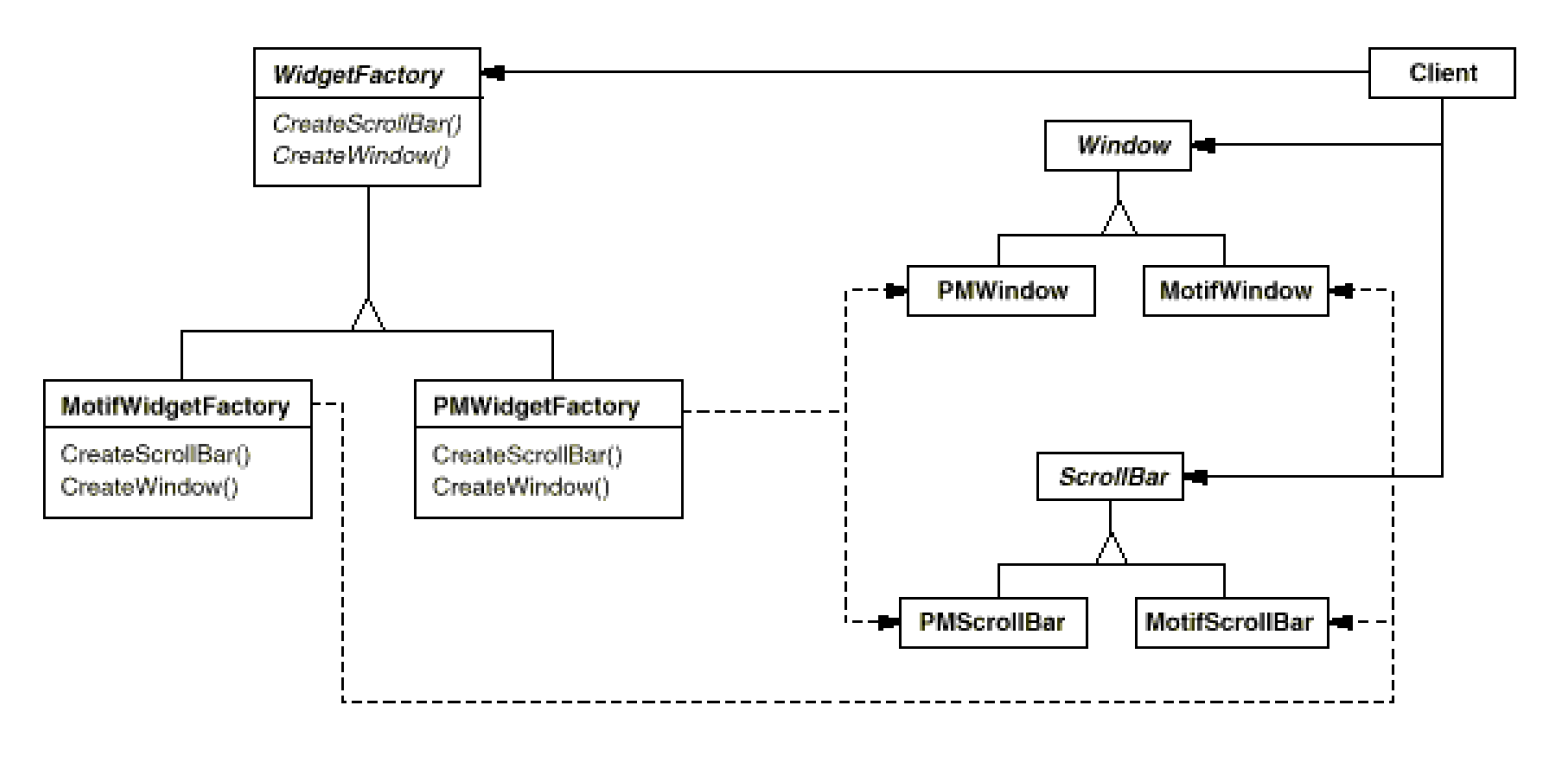
\includegraphics[scale=0.4]{motivation.png}
\end{center}
\end{frame}
%-------------------------------------------------------------------------------------------------

\subsection{Կիրառելիությունը}
%-------------------------------------------------------------------------------------------------
\begin{frame}\frametitle{Կիրառելիությունը}
Այս Ն.Ձ. պետք է օգտագործել երբ.
\vfill
\begin{enumerate}
    \item Կոմպլեքս օբյեկտ ստեղծելու ալգորիթմը պետք է անկախ լինի կառուցվելիք
    օբյեկտի մասերից, դրանց միավորման ձևից: \pause \vfill
    \item Կառուցման պրոցեսը պետք է թույլ տա կառուցվող օբյեկտի տարբեր ներկայացումներ:
\end{enumerate}
\end{frame}
%-------------------------------------------------------------------------------------------------

\section{Կառուցվածքը}
%-------------------------------------------------------------------------------------------------
\begin{frame}\frametitle{Կառուցվածքը}
\begin{center}
    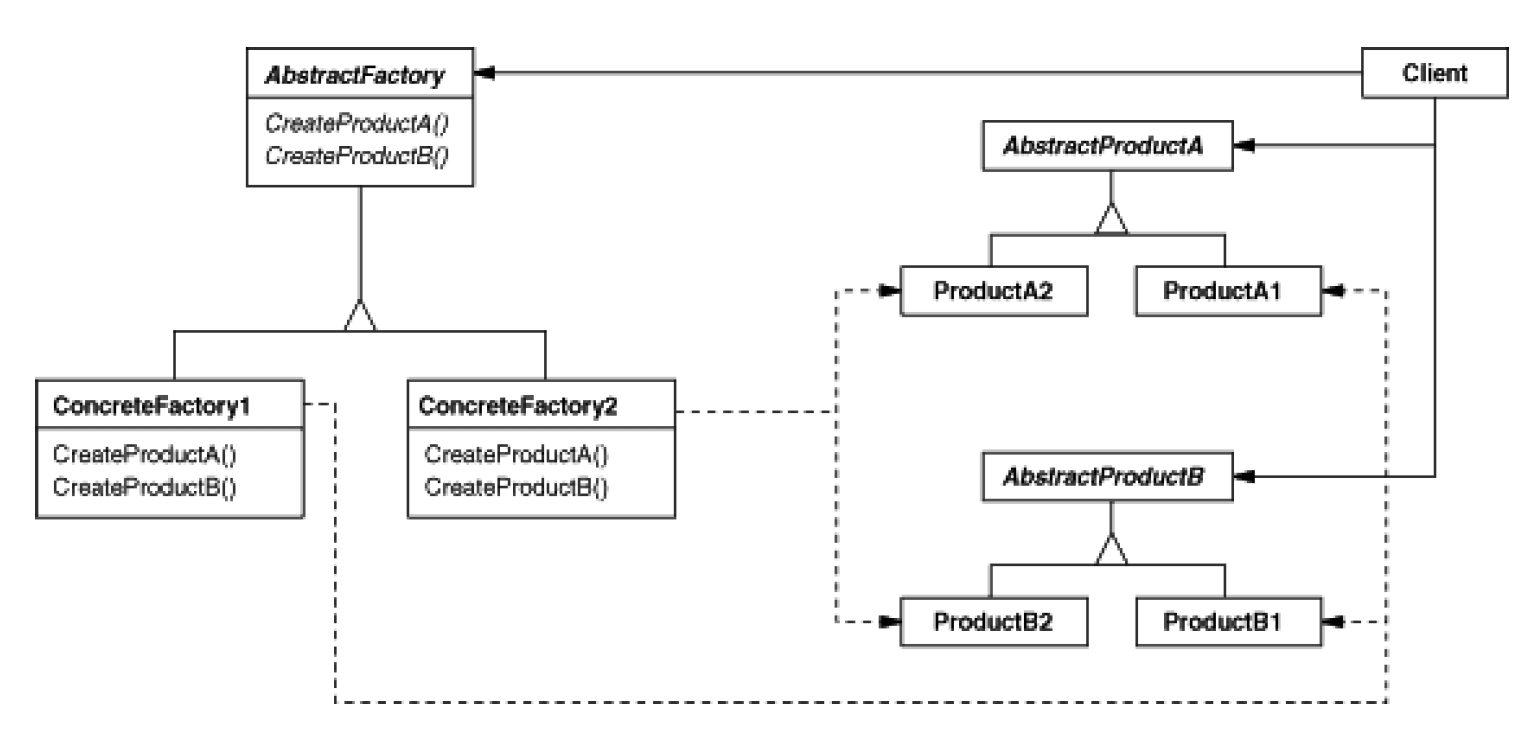
\includegraphics[scale=0.4]{structure.png}
\end{center}
\end{frame}
%-------------------------------------------------------------------------------------------------

%-------------------------------------------------------------------------------------------------
\begin{frame}\frametitle{Փոխհամագործակցությունը}
\begin{center}
    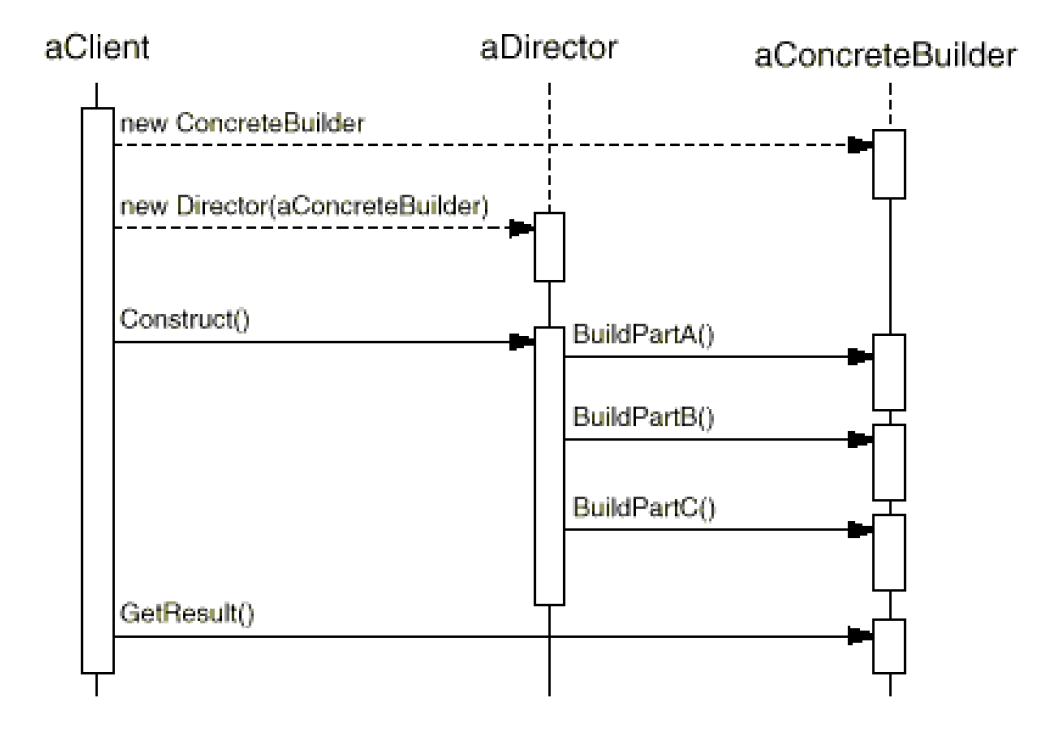
\includegraphics[scale=0.4]{collaborations.png}
\end{center}
\end{frame}
%-------------------------------------------------------------------------------------------------

\subsection{Հետևանքները}
%-------------------------------------------------------------------------------------------------
\begin{frame}\frametitle{Հետևանքները}
Այս Ն.Ձ. ունի հետևյալ առավելություններն ու թերությունները.
\vfill
\begin{enumerate}
    \item Թույլ է տալիս հեշտորեն փոփոխել օբյեկտների ներքին ներկայացումը: \pause \vfill
    \item Առանձնացնում է օբյեկտի կառուցման և ներկայացման կոդերը: \pause \vfill
    \item Տալիս է կառուցման պրոցեսի ավելի լավ ղեկավարման հնարավորություն:
\end{enumerate}
\end{frame}
%-------------------------------------------------------------------------------------------------

\section{Իրականացումը}
%-------------------------------------------------------------------------------------------------
\begin{frame}\frametitle{Իրականացումը}
\begin{enumerate}
    \item Կառուցման և միավորման ինտերֆեյս: \pause \vfill
    \item Ինչու ստեղծվելիք օբյեկտների համար աբստրակտ բազային դաս չի կիրառվում: \pause \vfill
    \item Դատարկ մեթոդներ աբստրակտ մեթոդների փոխարեն:
\end{enumerate}
\end{frame}
%-------------------------------------------------------------------------------------------------

\subsection{Օրինակ}
%-------------------------------------------------------------------------------------------------
\begin{frame}[fragile]\frametitle{Օրինակ}
\begin{english}
\begin{minted}{cpp}
class MazeBuilder {

public:
    virtual void BuildMaze() { }

    virtual void BuildRoom(int room) { }

    virtual void BuildDoor(int roomFrom, int roomTo) { }

    virtual Maze* GetMaze() { return 0; }

protected:
    MazeBuilder();
};
\end{minted}
\end{english}
\end{frame}
%-------------------------------------------------------------------------------------------------

%-------------------------------------------------------------------------------------------------
\begin{frame}[fragile]\frametitle{Օրինակ}
\begin{english}
\begin{minted}{cpp}
Maze* MazeGame::CreateMaze(MazeBuilder& builder) {

    builder.BuildMaze();

    builder.BuildRoom(1);

    builder.BuildRoom(2);

    builder.BuildDoor(1, 2);

    return builder.GetMaze();
}
\end{minted}
\end{english}
\end{frame}
%-------------------------------------------------------------------------------------------------

%-------------------------------------------------------------------------------------------------
\begin{frame}[fragile]\frametitle{Օրինակ}
\begin{english}
    \begin{minted}[fontsize=\scriptsize]{cpp}
        Maze* MazeGame::CreateMaze(MazeFactory& factory) {
            Maze* aMaze = factory.MakeMaze();

            Room* r1 = factory.MakeRoom(1);
            Room* r2 = factory.MakeRoom(2);
            aMaze->AddRoom(r1); aMaze->AddRoom(r2);

            Door* aDoor = factory.MakeDoor(r1, r2);
            r1->SetSide(East, aDoor); r2->SetSide(West, aDoor);

            r1->SetSide(North, factory.MakeWall());
            r1->SetSide(South, factory.MakeWall());
            r1->SetSide(West, factory.MakeWall());
            r2->SetSide(North, factory.MakeWall());
            r2->SetSide(East, factory.MakeWall());
            r2->SetSide(South, factory.MakeWall());

            return aMaze;
        }
    \end{minted}
\end{english}
\end{frame}
%-------------------------------------------------------------------------------------------------

%-------------------------------------------------------------------------------------------------
\begin{frame}[fragile]\frametitle{Օրինակ}
\begin{english}
\begin{minted}{cpp}
class StandardMazeBuilder : public MazeBuilder {

public:
    StandardMazeBuilder() { currentMaze_= NULL; }

    virtual void BuildMaze() { currentMaze_= new Maze; }

    virtual void BuildRoom(int);

    virtual void BuildDoor(int, int);

    virtual Maze* GetMaze() { return currentMaze_; }

private:
    Direction CommonWall(Room*, Room*);
    Maze* currentMaze_;
};
\end{minted}
\end{english}
\end{frame}
%-------------------------------------------------------------------------------------------------

%-------------------------------------------------------------------------------------------------
\begin{frame}[fragile]\frametitle{Օրինակ}
\begin{english}
\begin{minted}[fontsize=\scriptsize]{cpp}
void StandardMazeBuilder::BuildRoom(int n) {
    if (currentMaze_->RoomNo(n)) return;

    Room* room = new Room(n);
    currentMaze_->AddRoom(room);

    room->SetSide(North, new Wall); room->SetSide(South, new Wall);
    room->SetSide(East, new Wall); room->SetSide(West, new Wall);
}

void StandardMazeBuilder::BuildDoor(int n1, int n2) {
    Room* r1 = currentMaze_->RoomNo(n1);
    Room* r2 = currentMaze_->RoomNo(n2);

    Door* d = new Door(r1, r2);

    r1->SetSide(CommonWall(r1,r2), d);
    r2->SetSide(CommonWall(r2,r1), d);
}
\end{minted}
\end{english}
\end{frame}
%-------------------------------------------------------------------------------------------------

%-------------------------------------------------------------------------------------------------
\begin{frame}[fragile]\frametitle{Օրինակ}
\begin{english}
\begin{minted}{cpp}
Maze* maze;
MazeGame game;
StandardMazeBuilder builder;
game.CreateMaze(builder);
maze = builder.GetMaze();


Maze* maze;
MazeGame game;
StandardMazeFactory factory;
maze = game.CreateMaze(factory);
\end{minted}
\end{english}
\end{frame}
%-------------------------------------------------------------------------------------------------

%-------------------------------------------------------------------------------------------------
\begin{frame}[fragile]\frametitle{Օրինակ}
\begin{english}
\begin{minted}{cpp}
Maze* MazeGame::CreateComplexMaze(MazeBuilder& builder) {

    builder.BuildRoom(1);

    builder.BuildRoom(2);

    // ...

    builder.BuildRoom(1001);

    builder.BuildDoor(i1, i2);

    // ...

    return builder.GetMaze();
}
\end{minted}
\end{english}
\end{frame}
%-------------------------------------------------------------------------------------------------

%-------------------------------------------------------------------------------------------------
\begin{frame}[fragile]\frametitle{Օրինակ}
\begin{english}
\begin{minted}[fontsize=\scriptsize]{cpp}
class CountingMazeBuilder : public MazeBuilder {

public:
    CountingMazeBuilder(): doors_(0), rooms_(0) {}

    virtual void BuildMaze() { doors_ = rooms_ = 0;}

    virtual void BuildRoom(int) { ++rooms_;}

    virtual void BuildDoor(int, int) { ++doors_;}

    virtual void AddWall(int, Direction){}

    void GetCounts(int& doors, int& rooms) const {
        doors = doors_;  rooms = rooms_;
    }

private:
    int doors_; int rooms_;
};
\end{minted}
\end{english}
\end{frame}
%-------------------------------------------------------------------------------------------------

\section{Առնչվող Ձևանմուշները}
%-------------------------------------------------------------------------------------------------
\begin{frame}\frametitle{Առնչվող Նախագծման Ձևանմուշները}
\begin{itemize}
    \item Composite
\end{itemize}
\end{frame}
%-------------------------------------------------------------------------------------------------

\end{document}
